%%%%%%%%%%%%%%%%%%%%%%%%%%%%%%%%%%%%%%%%%
% Short Sectioned Assignment
% LaTeX Template
% Version 1.0 (5/5/12)
%
% This template has been downloaded from:
% http://www.LaTeXTemplates.com
%
% Original author:
% Frits Wenneker (http://www.howtotex.com)
%
% License:
% CC BY-NC-SA 3.0 (http://creativecommons.org/licenses/by-nc-sa/3.0/)
%
%%%%%%%%%%%%%%%%%%%%%%%%%%%%%%%%%%%%%%%%%

%----------------------------------------------------------------------------------------
%	PACKAGES AND OTHER DOCUMENT CONFIGURATIONS
%----------------------------------------------------------------------------------------

\documentclass[paper=a4, fontsize=11pt]{scrartcl} % A4 paper and 11pt font size
\usepackage[brazilian]{babel}
\usepackage[utf8]{inputenc}
\usepackage[T1]{fontenc}
\usepackage{amsmath,amsfonts,amsthm,mathtools} % Math packages
\usepackage{xspace}
\usepackage{indentfirst}
\usepackage{placeins}


\usepackage{tikz}
\usetikzlibrary{arrows}
\usetikzlibrary{positioning}
\usetikzlibrary{calc}

%\usepackage{sectsty} % Allows customizing section commands
%\allsectionsfont{\centering \normalfont\scshape} % Make all sections centered, the default font and small caps

\usepackage{fancyhdr}
\pagestyle{fancyplain}
%\fancyhead{}
\fancyfoot[L]{} % Empty left footer
\fancyfoot[C]{} % Empty center footer
\fancyfoot[R]{\thepage} % Page numbering for right footer
\renewcommand{\headrulewidth}{0pt} % Remove header underlines
\renewcommand{\footrulewidth}{0pt} % Remove footer underlines
\setlength{\headheight}{13.6pt} % Customize the height of the header

\bibliographystyle{apalike}

%\sectionfont{\bfseries\Large\raggedright}
%\subsectionfont{\bfseries\Large\raggedright}

\newtheorem{theorem}{Teorema}
\newtheorem{definition}{Definição}
\newtheorem{property}{Propriedade}
\newtheorem{proposition}{Proposição}

\newenvironment{example}[1][Exemplo]{\begin{trivlist}
\item[\hskip \labelsep {\bfseries #1}]}{\end{trivlist}}
\newenvironment{exerc}[1][Exercício]{\begin{trivlist}
\item[\hskip \labelsep {\bfseries #1}]}{\end{trivlist}}

\numberwithin{equation}{subsection}
\numberwithin{figure}{subsection}
\numberwithin{table}{subsection}
\numberwithin{definition}{subsection}
\numberwithin{theorem}{subsection}
\numberwithin{property}{subsection}
\numberwithin{proposition}{subsection}
%\numberwithin{example}{subsection}

\numberwithin{equation}{section}
\numberwithin{figure}{section}
\numberwithin{table}{section}
\numberwithin{definition}{section}
\numberwithin{theorem}{section}
\numberwithin{property}{section}
\numberwithin{proposition}{section}
%\numberwithin{example}{section}


% Default fixed font does not support bold face
\DeclareFixedFont{\ttb}{T1}{txtt}{bx}{n}{12} % for bold
\DeclareFixedFont{\ttm}{T1}{txtt}{m}{n}{12}  % for normal

% Custom colors
\usepackage{color}
\definecolor{deepblue}{rgb}{0,0,0.5}
\definecolor{deepred}{rgb}{0.6,0,0}
\definecolor{deepgreen}{rgb}{0,0.5,0}

\usepackage{listings}

% Python style for highlighting
\newcommand\pythonstyle{\lstset{
language=Python,
basicstyle=\ttm,
otherkeywords={self},             % Add keywords here
keywordstyle=\ttb\color{deepblue},
emph={MyClass,__init__},          % Custom highlighting
emphstyle=\ttb\color{deepred},    % Custom highlighting style
stringstyle=\color{deepgreen},
frame=tb,                         % Any extra options here
showstringspaces=false            % 
}}

% Python environment
\lstnewenvironment{python}[1][]
{
\pythonstyle
\lstset{#1}
}
{}


%\setlength{•}{•}\parindent{0pt} % Removes all indentation from paragraphs - comment this line for an assignment with lots of text

%----------------------------------------------------------------------------------------
%	TITLE SECTION
%----------------------------------------------------------------------------------------

\newcommand{\horrule}[1]{\rule{\linewidth}{#1}} % Create horizontal rule command with 1 argument of height

\title{	
\normalfont \normalsize 
\textsc{Modelos Probabilísticos Baseados em Grafos} \\ 
\textsc{Prof. Denis Mauá} \\ [25pt]
%\horrule{0.5pt} \\[0.4cm] % Thin top horizontal rule
\huge Redes Bayesianas \\ [25pt]
%\horrule{1pt} \\[0.5cm] % Thick bottom horizontal rule
}
\author{Thales A. B. Paiva \\ thalespaiva@gmail.com} % Your name
\date{\today} % Today's date or a custom date

\renewcommand{\P}{\mathbb{P}}
\renewcommand{\bar}[1]{\overline{#1}}
\newcommand{\set}[1]{\mathcal{#1}}

\begin{document}


\maketitle % Print the title
\horrule{1pt} \\[0.5cm] % Thick bottom horizontal rule

\tableofcontents


%----------------------------------------------------------------------------------------
%	PROBLEM 1
%----------------------------------------------------------------------------------------

\pagebreak
\section{Redes Bayesianas}

Redes Bayesianas são um meio de representar distribuições conjuntas que explora a independência entre variáveis para economizar espaço no armazenamento das informações. Para entender como essa independência é explorada, considere exemplo a seguir. Note que neste exemplo, por não ser esparso, a representação por redes bayesianas usa mais espaço.

\begin{example} Sejam Chuva, Sprinkler, e GramaMolhada variáveis que podem assumir os valores verdadeiro ou falso. Simbolicamente:
$$
dom(\text{Chuva}) = dom(\text{Sprinkler}) = dom(\text{GramaMolhada}) = \{V, F\}.
$$

A representação ingênua da distribuição conjunta dessas variáveis é dada pela Tabela~\ref{tab:rain_bayesnet}.
Note que, sob esta representação, precisamos de $7 = 2^{|V|} - 1$ valores, onde $V$ é o conjunto de variáveis (o oitavo é determinado por 1 menos a soma dos outros 7).
\begin{table}[]
\centering
\begin{tabular}{cccl}
\hline
\multicolumn{1}{l}{\textbf{GramaMolhada}} & \multicolumn{1}{l}{\textbf{Chuva}} & \multicolumn{1}{l}{\textbf{Sprinkler}} & \textbf{Probabilidade} \\ \hline
V                                         & V                                  & V                                      & 0.00198                \\
V                                         & V                                  & F                                      & 0.15840                \\
V                                         & F                                  & V                                      & 0.28800                \\
V                                         & F                                  & F                                      & 0.00000                \\
F                                         & V                                  & V                                      & 0.00002                \\
F                                         & V                                  & F                                      & 0.03960                \\
F                                         & F                                  & V                                      & 0.03200                \\
F                                         & F                                  & F                                      & 0.48000                \\ \hline
\end{tabular}
\caption{Representação ingênua da distribuição do exemplo da chuva.}
\label{tab:rain_bayesnet}
\end{table}

Para representar a distribuição com menor número de parâmetros, precisamos encontrar meios de relacioná-los. Uma forma de relacioná-los, é determinando dependências e independências.

É natural pensarmos que a probabilidade de o sprinkler ser acionado é menor quando chove do que quando não. É evidente que a grama estar molhada é altamente dependente dos eventos em que o sprinkler está ligado ou daquele em que chove. Estas relações estão representadas na Figura~\ref{fig:rain_bayesnet}, que pode ser gerada usando o programa enviado.


\begin{figure}[hbtp]
\centering
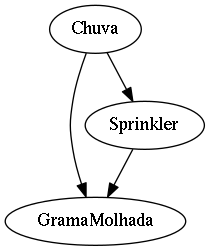
\includegraphics[scale=0.7]{images/rain_bayesnet.png}
\caption{Rede bayesiana que modela o problema da chuva.}
\end{figure}
\label{fig:rain_bayesnet}
\end{example} 

A força das redes bayesianas está no fato do teorema da fatorização que diz que:
$$
p(V) = \prod_{X \in V} p(X|pa(X)).
$$

\section{Resolução dos Exercícios}

\begin{exerc}
Compute o número de valores de probabilidade necessário para especificar uma Rede Bayesiana em forma de árvore com $n$ variáveis binárias.

A menos da raíz, todo nó tem um só pai. Cada nó não raiz tem as suas probabilidades determinadas ao especificar $\P(X|pai(X))$ e $\P(X|\neg pai(X))$, mas não as tem com menos do que isso. A raiz precisa especificar apenas um dos valores. Assim, o número de valores de probabilidades é $2(n - 1) + 1 = 2n - 1$. 
\end{exerc}

\begin{exerc}
Compute o número de valores de probabilidade necessários para especificar uma Rede Bayesiana bipartida com m variáveis raízes (binárias)e n folhas (ternárias). \emph{Obs: não ficou claro qual o grau considerado para os nós. Então considerei que se tratava de uma rede bipartida completa (há um arco de toda raiz para toda folha.}

Cada raiz deve especificar apenas um valor. Cada folha deve especificar no máximo (no caso em que temos um bipartido completo) $2.2^m = 2^{m+1}$ valores. Assim, no pior caso, ou seja, o menos esparso, precisamos especificar $n2^{m+1} + m$ valores.
\end{exerc}

\begin{exerc}
Prove que as folhas de uma Rede de Bayes ingênua são duas a duas independentes.

\end{exerc}

\pagebreak  
\section{Implementação em Python: \texttt{bayesnet.py}}

Implementei em Python um parser de descrições no formato BIF. Não tive muita dificuldade pois no site do Professor Cozman, a gramática já estava definida. Usei a biblioteca \verb|pyparsing| para poder descrever a gramática e as ações de parsing em Python, deixando o programa mais simples e sem precisar recorrer a outras sintaxes. A classe responsável pelo parsing é chamada \verb|BIF_parser| e seus métodos são:

\begin{python}
class BIF_Parser:
  def parse(file_path)
  def _get_variable_from_data_item(item)
  def _get_prob_from_data_item(item, variables)
\end{python}

Para representar redes bayesianas, escrevi a classe \verb|BayesNet|. Instâncias dessa classe têm nome, uma coleção de nós (que representam as variáveis), uma coleção de distribuição de probabilidades (uma distribuição condicional para cada variável, como descrito no arquivo de entrada). Seus métodos são:

\begin{python}
class BayesNet:
  def __init__(self, name, nodes, probs, properties=None)
  def parent_nodes(self, node_name)
  def init_from_bif_file(bif_file_path)
  def draw(self, file_path)
  def get_var_distribution(self, var_name)
  def get_ancestors_set(self, nodes)
  def get_joint_distribution(self, variables_names)
  def conjunctive_query(self, valuation)
\end{python}

Seus métodos mais interessantes são \verb|get_joint_distribution| e \verb|conjunctive_query|, inclusive a segunda faz uma chamada à primeira. O método draw foi usado apenas para testar se o parser estava funcionando corretamente. O desenho da rede Asia lida é dado na Figura~\ref{fig:asianet}.

\begin{figure}[hbtp]
\centering
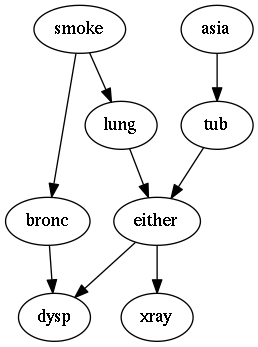
\includegraphics[scale=0.7]{images/asianet.png}
\caption{Rede bayesiana lida para a entrada \texttt{asia.bif}.}
\label{fig:asianet}
\end{figure}

Para implementar a álgebra de funções para distribuições, escrevi as classes \verb|Function| e \verb|Probability|. A primeira é superclasse da segunda, e enquanto a primeira guarda apenas as variáveis, a segunda guarda separadamente variáveis principais e condicionais. O que chamo de principais são aquelas que vêm antes da barra vertical na declaração de uma variável condicional (e.g. em $\P(A, B| C, D)$, A e B são principais, e C e D são condicionais. Essa distinção é importante pelo modo como elas fazem eliminação de variáveis.

Implementei todas as operações da álgebra através de métodos mágicos do python. Se \verb|p| e \verb|q| são instâncias da classe \verb|Probability| e \verb|v| é uma \verb|Variable|, então: \verb|p * q| faz o produto das funções de probabilidade, \verb|p / q| faz a divisão, e \verb|p % v| faz a eliminação da variável de nome \verb|v| de \verb|p|. Note também que cada uma das operações retorna um novo objeto de \verb|Probability| (ou \verb|Function|).

A interface dessas classes é:

\begin{python}
class Function:
    def __init__(self, variables)
    def add_value(self, valuation, value)
    def __str__(self)
    def evaluate(self, var_valuation)
    def __mul__(self, function)
    def __div__(self, function)
    def __sub__(self, variable)
class Probability(Function):
    def __init__(self, main_vars, cond_vars)
    def __mod__(self, variable)
    def __mul__(self, probab)
    def __div__(self, probab)
\end{python}

Abaixo pode-se ver alguns exemplos de uso, rodando o módulo sobre o ipython. Esse também é o main chamado quando se roda \verb|./bayesnet.py|.

\begin{verbatim}
$ ipython -i bayesnet.py
In []: p, q = asia.probs['lung'], asia.probs['xray']
In []: print(p)
[F] F over ['lung', 'smoke']
    ('yes', 'yes')            :    0.10000
    ('yes', 'no')             :    0.01000
    ('no', 'yes')             :    0.90000
    ('no', 'no')              :    0.99000 
In []: print(q)
[F] F over ['xray', 'either']
    ('yes', 'yes')            :    0.98000
    ('yes', 'no')             :    0.05000
    ('no', 'yes')             :    0.02000
    ('no', 'no')              :    0.95000
In []: r = p * q
In []: print(r)
[F] F over ['xray', 'lung', 'either', 'smoke']
    ('yes', 'yes', 'yes', 'yes') :    0.09800
    ('yes', 'yes', 'yes', 'no') :    0.00980
    ('yes', 'yes', 'no', 'yes') :    0.00500
    ('yes', 'yes', 'no', 'no') :    0.00050
    ('yes', 'no', 'yes', 'yes') :    0.88200
    ('yes', 'no', 'yes', 'no') :    0.97020
    ('yes', 'no', 'no', 'yes') :    0.04500
    ('yes', 'no', 'no', 'no') :    0.04950
    ('no', 'yes', 'yes', 'yes') :    0.00200
    ('no', 'yes', 'yes', 'no') :    0.00020
    ('no', 'yes', 'no', 'yes') :    0.09500
    ('no', 'yes', 'no', 'no') :    0.00950
    ('no', 'no', 'yes', 'yes') :    0.01800
    ('no', 'no', 'yes', 'no') :    0.01980
    ('no', 'no', 'no', 'yes') :    0.85500
    ('no', 'no', 'no', 'no')  :    0.94050
In []: v = asia.nodes['smoke']
In []: z = r % v
In []: print(z)
[F] F over ['xray', 'lung', 'either']
    ('yes', 'yes', 'yes')     :    0.02695
    ('yes', 'yes', 'no')      :    0.00138
    ('yes', 'no', 'yes')      :    0.46305
    ('yes', 'no', 'no')       :    0.02363
    ('no', 'yes', 'yes')      :    0.00055
    ('no', 'yes', 'no')       :    0.02613
    ('no', 'no', 'yes')       :    0.00945
    ('no', 'no', 'no')        :    0.44888
\end{verbatim}

Para representar as funções, usei dicionários que mapeiam valorações das variáveis a valores de probabilidades. Para percorrer as valorações, usei os iteradores do módulo \verb|itertools|, principalmente o \verb|product| para fazer produtos cartesianos de domínios sob demanda.

Para fazer buscas conjuntivas, use o método \verb|conjunctive_query|. Por exemplo, da página 77 do livro do Darwiche, se quisermos saber a probabilidade de dar raio-X positivo sem dispneia (que, pelo livro, deve ser de aproximadamente 3.96\%), pode-se fazer:

\begin{verbatim}
In [31]: valuation = {'xray': 'yes', 'dysp': 'no'}
In [32]: asia.conjunctive_query(valuation)
Out[32]: 0.0396199356
\end{verbatim} 

\end{document}